%********************************************************************
% Appendix
%*******************************************************
\chapter{Anhang -Kundenverwaltung}

\section{Kundenerfassung}
Hier kann man besser sehen wie die Umsetzungsvorgabe erfüllt wurde.

Im Model werden die Attributen erstellt, die von den Cotroller und PartialView benutzt werden.

\begin{lstlisting}[caption={RegisterModel}, label=lst:registerModel]
using System.ComponentModel.DataAnnotations;

namespace newKonzept.Models.Register
{
	public class RegisterModell
	{
		[Required]
		public string Name { get; set; }
		[Required]
		public string Vornane { get; set; }
		[Required]
		public string Ort { get; set; }
		[Required]
		[EmailAddress]
		public string Email { get; set; }
		public string Password { get; set; }
	}
}
\end{lstlisting}

 Im "PartialView" werden vom Model und PIN JavaScript-Funktion-Generator angegeben, die Attribute von Model. 

\begin{lstlisting}[caption={RegisterView}, label=lst:RegisterView]

@model newKonzept.Models.Register.RegisterModell
@using newKonzept.Controllers.Register;


@if (TempData["success"] == null)
{
	using (Html.BeginUmbracoForm<CheckIsApprovedController>("HandleFormSubmit"))
	{
		using (Html.BeginUmbracoForm<RegisterController>("Register"))
		{
			
			@Html.AntiForgeryToken()
			@Html.ValidationSummary(true)
			
			<fieldset>
			<div class="row form-group">
			<div class="col-md-6">
			<!-- <label for="lname">Last Name</label> -->
			@Html.TextBoxFor(m => m.Name, new { @class = "form-control", placeholder = "Name" })
			@Html.ValidationMessageFor(m => m.Name)
			
			</div>
			</div>
			
			<div class="row form-group">
			<div class="col-md-6">
			<!-- <label for="lname">Last Name</label> -->
			@Html.TextBoxFor(m => m.Vornane, new { @class = "form-control", placeholder = "Vorname" })
			@Html.ValidationMessageFor(m => m.Vornane)
			
			</div>
			</div>
			
			<div class="row form-group">
			<div class="col-md-6">
			<!-- <label for="email">Email</label> -->
			@Html.TextBoxFor(m => m.Email, new { @class = "form-control", placeholder = "Email" })
			@Html.ValidationMessageFor(m => m.Email)
			</div>
			</div>
			<div class="row form-group">
			<div class="col-md-6">
			<!-- <label for="lname">Last Name</label> -->
			@Html.TextBoxFor(m => m.Ort, new { @class = "form-control", placeholder = "Ort" })
			@Html.ValidationMessageFor(m => m.Ort)
			
			</div>
			</div>
			@Html.HiddenFor(m => m.Password, new { id = "newInput", Value = "123" })
			@Html.ValidationMessageFor(m => m.Password)
			@section Scripts{
				
				<script type="text/javascript" src="~/Scripts/randomNr.js"></script>
			}
			
			<div class="form-group">
			<button type="submit" class="btn btn-primary">Register</button>
			</div>
			
			
			</fieldset>
			
		}
		
	}
}
else
{
	<p>Sie haben sich erfolreich registriert!</p>
}

\end{lstlisting}

PIN JavaScript-Generator. der PIN wird werden zwischen den Zahlen 1000 und 9999 generiert.

\begin{lstlisting}[caption={PIN-Generator}, label=lst:PIN-Generator]
function myFunction() {
	document.getElementById('newInput').setAttribute('Value', Math.floor((Math.random() * 9000) + 1000));
}window.onload = myFunction;

\end{lstlisting}
Der Kunde gibt seine Daten ein.

\begin{figure}[h]
	\centering
	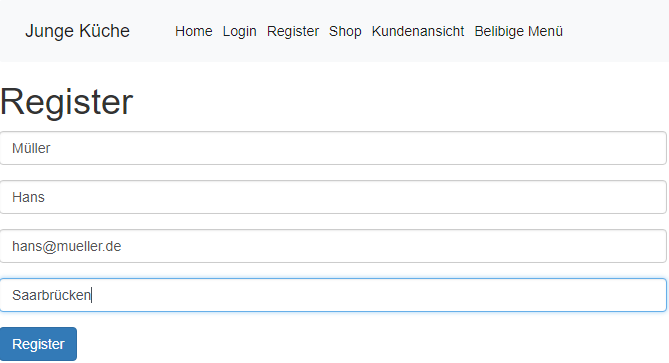
\includegraphics[width=1\linewidth]{Graphics/newRegister.png}
	\caption[newRegister]{Der Kunde gibt seine Daten ein.}
	\label{fig: newRegister}
\end{figure}

Die eingegebene Daten werden über SurfaceController zum Umbraco Databank zu geschickt.


\begin{lstlisting}[caption={RegisterConsontroller}, label=lst:RegisterConsontroller]
using System.Web.Mvc;
using Umbraco.Web.Mvc;
using newKonzept.Models.Register;

namespace newKonzept.Controllers.Register
{
	public class RegisterController : SurfaceController
	{
	// GET: Register
		public ActionResult Register(RegisterModell model)
		{
			if (!ModelState.IsValid)
			{
				return CurrentUmbracoPage();
			}

			var memberService = Services.MemberService;

			if (memberService.GetByEmail(model.Email) != null)
			{
				ModelState.AddModelError("", "Mietglider/in mit diesem Konte schon existiert!");
				return CurrentUmbracoPage();
			}

			//Schick die Information an Umbraco
			var member = memberService.CreateMemberWithIdentity(model.Email, model.Email, model.Name, "neueKunden");
			member.SetValue("ort", model.Ort);
			member.SetValue("password", model.Password);
			member.IsApproved = false;
			memberService.AssignRole(member.Username, "Normal");
			memberService.SavePassword(member, model.Password);
			Members.Login(model.Email, model.Password);
			memberService.Save(member);

			return Redirect("/");
		}
	}
}
\end{lstlisting}

Der Kunde ist mit automatisch generierter PIN im Umbraco Member-Section gespeichert. Jetzt wartet der Kunde auf die Bestätigung.

\begin{figure}[h]
	\centering
	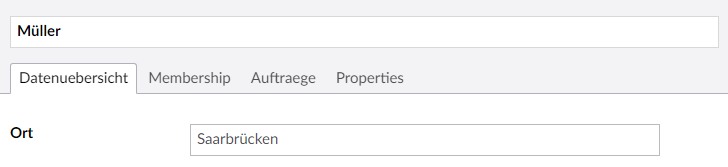
\includegraphics[width=1\linewidth]{Graphics/MemberDatenuebersicht.png}
	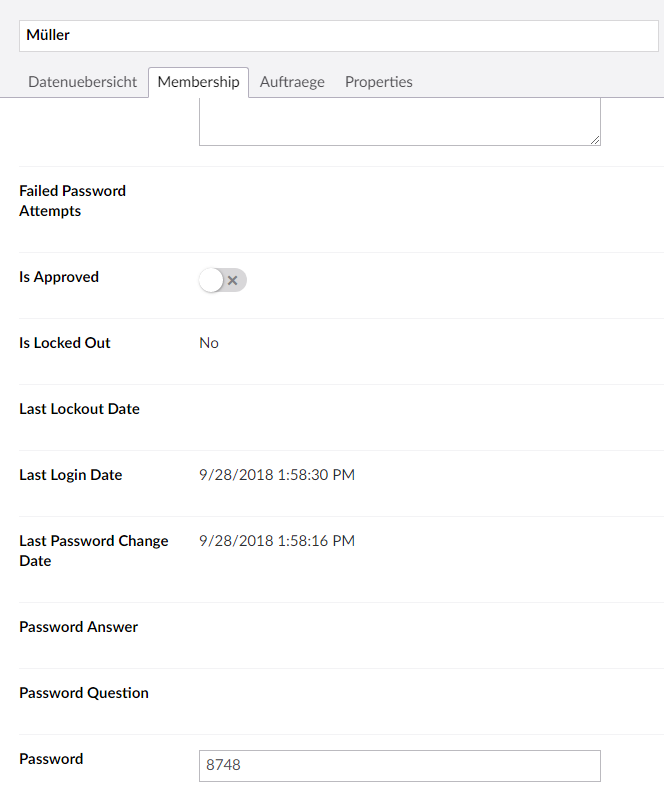
\includegraphics[width=1\linewidth]{Graphics/MemberMembership.png}
	\caption[MemberDatenuebersicht]{Die Kunde im Members gespeichert.}
	\label{fig: MemberDatenuebersicht}
\end{figure}

\newpage

\section{Kundenansicht}
\begin{lstlisting}[caption={Class E-Mail zum Kunde schicken}, label=lst:EmailSchicken]

namespace newKonzept.Controllers.Register
{
public class CheckIsApprovedController : SurfaceController
{
// GET: CheckIsApproved

public ActionResult Index()
{
return PartialView("RegisterPartial", new RegisterModell());
}		

[HttpPost]
public ActionResult HandleFormSubmit(RegisterModell model)
{
void MemberService_Saving(IMemberService sender, SaveEventArgs<IMember> e)
{
foreach (IMember umbMember in e.SavedEntities)
{

if (!umbMember.IsApproved)
{
continue;
}

bool oldValue = ApplicationContext.Current.Services.MemberService.GetById(umbMember.Id).IsApproved;

if (oldValue != umbMember.IsApproved)
{
MailMessage message = new MailMessage();
message.To.Add(model.Email);
message.Subject = "PIN";
message.From = new System.Net.Mail.MailAddress("office@jungekueche.com");
message.Body = model.Password;
SmtpClient smtp = new SmtpClient();
smtp.Send(message);
}
}
}
return RedirectToCurrentUmbracoPage();
}
}
}
\end{lstlisting}

\newpage
\section{Anhang - Auftraggeber-Ansicht}

\begin{lstlisting}[caption={Migrationsclass}, label=lst:migrationsController]

using System;
using System.IO;
using System.Web.Mvc;
using Umbraco.Core.Models;
using Umbraco.Web.Mvc;

namespace newKonzept.Controllers.MemberController
{
public class MemberController : SurfaceController
{
// GET: Member
public ActionResult ImportMembers()
{
string _line = "";
using (StreamReader sr = new StreamReader(System.Web.HttpContext.Current.Server.MapPath("~/DtenbankDatei.csv")))
{
do
{
//Liest die Reihe vom CSV-Datei
_line = sr.ReadLine();

//Prueft, ob die Reihe leer ist.
if (!String.IsNullOrEmpty(_line))
{
//trennt die Reihen mithilfe von ;-Zeichen
string[] _splits = _line.Split(';');

if (_splits.Length == 8)  //Die Zahl hier ist gleich von den Zahl der angegebenen Attribute in der alten Datenbank
{
//Die Zahlen im _splits[] zeigen die Positionen, in denen sich zugehoeriges Attribut in der altenDatenbank befindet
//Estellt neues Member
IMember member = Services.MemberService.CreateMember(
_splits[3],     // Username
_splits[2],     // Email
_splits[6],     // Display name
"neueKunden"    // Member type
);

//Member ist bestaetigt zu Login
member.IsApproved = true;

//Prueft, ob zugehoeriges Attribut existiert im Member-Section und dann sezt den Wert ein.
if (member.HasProperty("nameDesProperty"))
member.SetValue("nameDesProperty", _splits[4]);


if (member.HasProperty("nameDesProperty") && !String.IsNullOrEmpty(_splits[5]))
member.SetValue("nameDesProperty", _splits[5]);


if (member.HasProperty("nameDesProperty"))
member.SetValue("nameDesProperty", _splits[0]);


if (member.HasProperty("nameDesProperty"))
member.SetValue("nameDesProperty", _splits[1]);

try
{

//Spechert Member
Services.MemberService.Save(member);

//Speichert PIN des Members
Services.MemberService.SavePassword(member, _splits[7]);

//Korrekte Role zuweisen
Services.MemberService.AssignRole(member.Id, "MemberRole");

}
catch { }
}
}
} while (!sr.EndOfStream);

}

return null;

}
}
}
\end{lstlisting}